\section{Experimental Setup and Implementation}
\subsection{Compiled Updates}
Numba compiles the reference accumulations and linear solves. Users update independently with movies fixed, followed by the movie phase; parallel iterations write separate parameter rows \citep{numbaParallel}. Ratings use float32, while parameters and accumulated errors use float64. Batched evaluation avoids allocating a ratings-by-factors matrix. Per-sweep complexity is $O(|T|K^2+(M+N)K^3)$.

The recorded Linux run used Python 3.13, NumPy 2.1, and Numba 0.61, with two Numba threads and one BLAS thread. Table~\ref{tab:benchmark} compares identical starting parameters after compilation warmup and verifies agreement with the reference. Compilation supplies the main speedup; parallel scheduling adds overhead on this bounded workload.

\begin{table}[H]
\caption{One user-side update on 64,301 ratings, $K=10$. Medians of three timings after warmup.}
\label{tab:benchmark}\centering\small\begin{tabular*}{\linewidth}{@{\extracolsep{\fill}}lrr}
\toprule
Method & Median (ms) & Speedup \\
\midrule
Python reference & 811.34 & 1.00$\times$ \\
Numba serial & 14.85 & 54.64$\times$ \\
Numba parallel & 15.34 & 52.91$\times$ \\
\bottomrule
\end{tabular*}

\end{table}

\subsection{Evaluation Protocol}
Seed 42 assigns each rating to training with probability 0.8 (Table~\ref{tab:data}). Updates use training data only. There is no validation set. Test RMSE is monitored, but factor models retain sweep 20 without early stopping or checkpoint selection.

The baseline fixes $K=10$, $\lambda=0.01$, $\tau_b=0.001$, and $\tau=0.1$. Comparisons change one setting: $K=20$, $\tau=0.01$, $\tau=1$, or $\lambda=0.1$. Genre ALS adds $\eta=0.1$. Baseline settings also supply the genre and full-data refits; separate $K=2$ models produce the embeddings.

For test observations $S$, evaluate unclipped predictions using
\begin{equation}
\operatorname{RMSE}(S)=\sqrt{\frac{1}{|S|}\sum_{(m,n)\in S}(r_{mn}-\widehat r_{mn})^2}.
\end{equation}
Metrics are reported to two decimals; full-precision values remain in the result CSVs. Hyperparameters retain their exact values. The monitored test set is not an untouched final holdout.

\subsection{Bias-History Correction}
The bias run contains eight updates followed by twenty more with a restarted counter. Independent fitting reproduces all 28 updates. Figure~\ref{fig:bias} corrects only the cumulative-update axis; factor models still use 20 sweeps.

\begin{figure}[H]
\centering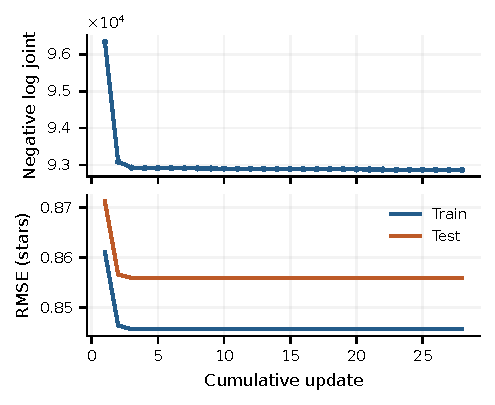
\includegraphics[width=\columnwidth]{bias_learning_curves.pdf}
\caption{Bias fitting over 28 verified updates. The plotted objective is the negative log joint, $\mathcal J_B=-\mathcal L_B$.}
\label{fig:bias}\end{figure}
